\documentclass[dvipsnames]{beamer}
\usepackage{lmodern}
\usepackage{appendixnumberbeamer}
\renewcommand{\sfdefault}{lmss}
\renewcommand{\ttdefault}{lmtt}
\usepackage[T1]{fontenc}
% \usepackage[utf8]{inputenc}
\setcounter{secnumdepth}{3}
\setcounter{tocdepth}{3}
\usepackage{amsmath}
\usepackage{amsthm}
\usepackage{amssymb}
\theoremstyle{definition}
\newtheorem*{defn*}{\protect\definitionname}
\providecommand{\definitionname}{Definition}
\usepackage{graphicx}
\usepackage{hyperref}
\usepackage{ulem}
\PassOptionsToPackage{normalem}{ulem}
\usepackage{caption}
\usepackage{subcaption}
\usepackage{verbatim}
\usepackage[english]{babel}
\usepackage[autostyle]{csquotes}
\usepackage{tikz}
\usetikzlibrary{arrows,intersections}
\usepackage{pgfplots}
\pgfplotsset{compat = 1.15}
\usepgfplotslibrary{fillbetween}
\usepackage{verbatim}
\usepackage{booktabs}
\usepackage{multirow}
\usepackage{array}
\usepackage{nccmath}
% \usepackage{listings}
\usepackage{mathtools}

%Bibliography style, etc.
\usepackage[citestyle=authoryear-comp,natbib, uniquename = false, url = false, doi = false, uniquelist=false]{biblatex}
\renewbibmacro{in:}{}
\AtEveryBibitem{%
  \clearfield{volume}%
  \clearfield{number}
  \clearfield{month}
  \clearfield{issn}
  \clearfield{isbn}
  \clearfield{pages}
}

%\usepackage{cleveref}
\usepackage{setspace}
\makeatletter

% Macros
\providecommand{\tabularnewline}{\\}
\newcommand{\gr}{\textcolor{ForestGreen}} 
\newcommand{\rd}{\textcolor{red}}
\newcommand{\cb}{\textcolor{CornflowerBlue}} %this is the blue color you like; simply type \cb{X} where "X" is the color you want in blue
\newcommand{\vitem}{\vfill \item} %auto-centers items in lists
\newcommand{\fall}{\ \forall} %redefines "forall" (I don't like the default spacing)
\newcommand{\frall}{\quad \forall} %a \forall separated from the main math; this is the way it usually shows up in equations
\newcommand{\exist}{\ \exists} %same as \fall, but for \exists; they have the same ugly spacing
\newcommand{\R}{\mathbb{R}} %set of real numbers
\newcommand*\bigcdot{\mathpalette\bigcdot@{.5}} %different size for cdots
% \newcommand{\argmax}{\text{arg}\max}
\newenvironment{itemframe}
    {\frame{}\itemize}
    {\itemize\frame}
\newcommand\makebeamertitle{\frame{\maketitle}}%
\newtheoremstyle{named}{}{}{\itshape}{}{\bfseries}{.}{.5em}{\thmnote{#3's }#1}
\theoremstyle{named}
\newtheorem*{prop*}{Proposition}
% \newtheorem*{corollary}{Corollary}
\newtheorem*{namedtheorem}{Theorem} %allows named theorems
\newtheorem*{nameddef}{Definition}
\newtheorem{proposition}{Proposition}
\newtheorem*{assumption}{Assumption}
\newtheorem*{namedcorollary}{Corollary}
\newtheorem*{namedlemma}{Lemma}
\newtheorem*{axiom}{Axiom}
\newtheorem*{theorem*}{Theorem}
\newtheorem*{lemma*}{Lemma}
\DeclareMathOperator*{\argmin}{argmin}
\DeclareMathOperator{\argmax}{argmax}
\DeclareMathOperator{\supp}{supp}
\DeclareMathOperator{\interior}{int}
\DeclareMathOperator{\rank}{rank}
\newcolumntype{C}[1]{>{\centering\let\newline\\\arraybackslash\hspace{0pt}}m{#1}}
\newcommand{\sbt}{\,\begin{picture}(-1,1)(-1,-3)\circle*{2}\end{picture}\ }



%formatting
\usetheme{Ilmenau}
\definecolor{MIT}{rgb}{.639,.122,.204}
\definecolor{UCLA}{rgb}{0.15294117647058825, 0.4549019607843137, 0.6823529411764706}
\definecolor{UCLA_gold}{rgb}{1, 0.8196078431372549, 0}
\usecolortheme[named=UCLA]{structure}
\setbeamercolor*{palette secondary}{fg=UCLA_gold,bg=gray!15!white}
\usecolortheme{dolphin}
\setbeamertemplate{navigation symbols}{} 
\setbeamertemplate{footline}{}{}
\setbeamertemplate{headline}{}
\setbeamertemplate{navigation symbols}{}
\mode<presentation> {}
\setbeamercolor{block title}{use=structure,fg=white,bg=RoyalBlue} %blocks (theorems, etc.)in blue
\setbeamercolor{block title alerted}{use=structure,fg=white,bg=ForestGreen} %blocks (theorems, etc.)in blue

\renewcommand\qedsymbol{$\blacksquare$} %set QED symbol as black square
\renewcommand{\emph}{\textit} %set emphasized text style; this is italics
\setbeamertemplate{footline}[frame number] %slide numbers
\setbeamertemplate{itemize item}[circle] %bullet style
\setbeamertemplate{itemize subitem}{--}
\setbeamertemplate{enumerate item}[default]
\newrobustcmd*{\parentexttrack}[1]{%
  \begingroup
  \blx@blxinit
  \blx@setsfcodes
  \blx@bibopenparen#1\blx@bibcloseparen
  \endgroup}

\AtEveryCite{%
  \let\parentext=\parentexttrack%
  \let\bibopenparen=\bibopenbracket%
  \let\bibcloseparen=\bibclosebracket}

 \AtBeginDocument{%
   \let\origtableofcontents=\tableofcontents
   \def\tableofcontents{\@ifnextchar[{\origtableofcontents}{\gobbletableofcontents}}
   \def\gobbletableofcontents#1{\origtableofcontents}
 }
\newcommand{\backupbegin}{
   \newcounter{framenumberappendix}
   \setcounter{framenumberappendix}{\value{framenumber}}
}
\newcommand{\backupend}{
   \addtocounter{framenumberappendix}{-\value{framenumber}}
   \addtocounter{framenumber}{\value{framenumberappendix}} 
} 

\renewcommand{\maketitle}{
\setbeamertemplate{footline}{} 
\begin{frame}[noframenumbering]
\titlepage
\end{frame}
\setbeamertemplate{footline}[frame number]
}

\usefonttheme[onlymath]{serif}

% \usetheme{CambridgeUS}

% \newtheorem{theorem}{Theorem}
% \theoremstyle{claim}
\newtheorem{claim}{Claim}
% \newtheorem{corollary}{Corollary}


\makeatother


%\author{Drew Fudenberg}

\institute[]{}

\begin{document}
% \maketitle
\begin{frame}{Overview}
  \begin{itemize}
  \item Are RTE cereal firms colluding?
    \begin{itemize}
    \item Existing evidence says probably yes (FTC case in the 1970s; Schmalensee 1978)
    \end{itemize}
    \vitem Consumers spend $\sim 9$B/year on cereal (wow) and firms make $\sim 3$B in profits 
\vitem Nevo models demand for cereals, then tests different market structures for suppliers to see which most closely matches firm behavior in the data
% \item Needs to use a more flexible model than logit to accurately model substitution patterns
  % \begin{itemize}
  % \item We think that Lucky Charms and Froot Loops are closer substitutes than Raisin Bran and Froot Loops
  % \end{itemize}
  \end{itemize}
\end{frame}
%
\begin{frame}{Why do we think RTE firms are colluding?}
  \begin{center}
 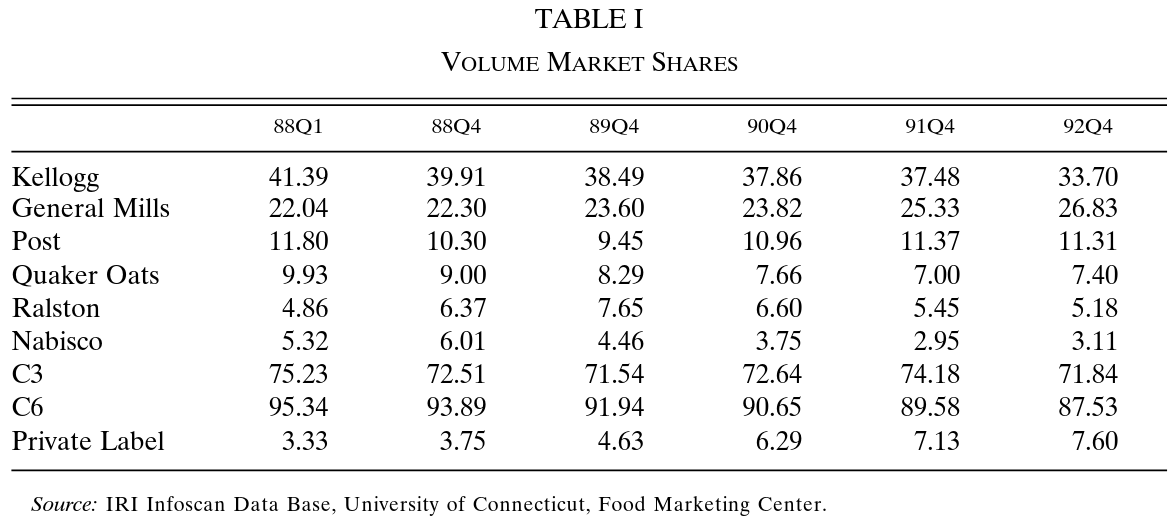
\includegraphics[width=.8\textwidth, keepaspectratio=true]{tab1.png} 
 \\
 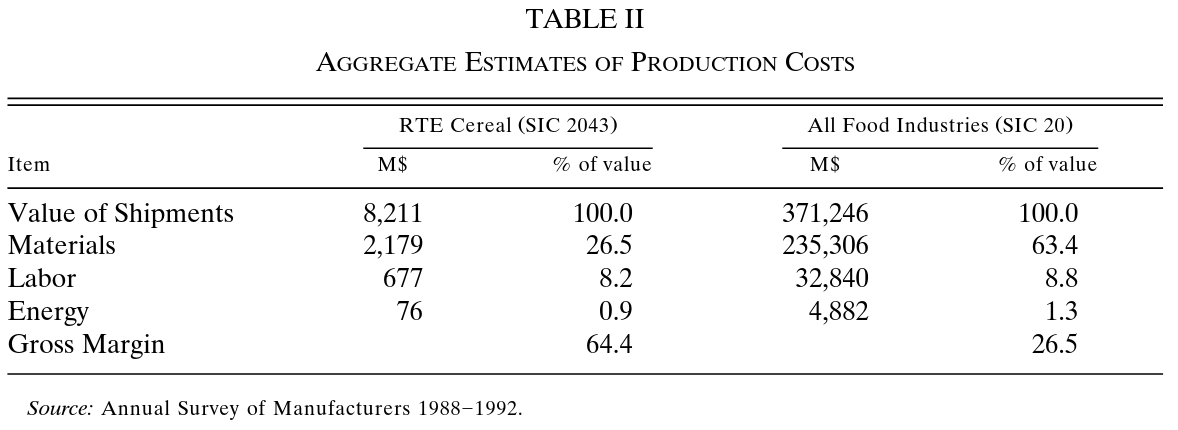
\includegraphics[width=.8\textwidth, keepaspectratio=true]{tab2.png} 
 \end{center}
\end{frame}
\begin{frame}{Approach (Supply)}
  \begin{itemize}
  \item Trying to answer the question ``Are RTE cereal firms colluding?''
  \vitem We know that there are different FOCs for different models of supply.
  \vitem Essentially the question is ``Can we reject that firms are acting like profit-maximizing colluders?''
  \vitem Can write FOCs as
    \[
      s_j (p) + \gr{\sum_{r \in \mathcal{F}_f}} (p_r - mc_r) \frac{\partial s_r(p)}{\partial p_j} = 0.
\]
\item The important bit is $\gr{\sum_{r \in \mathcal{F}_f}}$; firms are only looking at the products that they produce, and this is what's changing when we look at different supply side models.
  \end{itemize}
 \end{frame}
 %
 \begin{frame}{Approach (Supply)}
   \begin{itemize}
   \item Demand estimates let us estimate price-cost margins without seeing costs.
     \item Look at three different models for the supply side
     \begin{enumerate}
     \item Single-product firms
       \item Multi-product firms (existing structure)
       \item Monopoly/perfect price collusion
     \end{enumerate}
   \vitem Looking at these three different models of supply lets us distinguish between three different causes of markups:
     \begin{enumerate}
     \item Product Differentiation
       \item Portfolio effect
       \item Price collusion
     \end{enumerate}
   \end{itemize}
 \end{frame}
% 
 \begin{frame}{Approach (Demand)}
   \begin{itemize}
   \item The exercise on the supply-side depends on own- and cross-price elasticities; we need to estimate these.
   \item Consumer Utility:
     \begin{align*}
       u_{ijt} &= \underbrace{\delta_{jt}(x_j, p_{jt}, \xi_{jt}; \theta_1)}_{\text{mean utility}} + \underbrace{\mu_{ijt}(x_j, p_{jt}, \nu_j, D_i; \theta_2) + \epsilon_{ijt}}_{\text{mean-zero deviation}} \\
       \delta_{jt} &= x_j \beta - \alpha p_{jt} + \xi_{j} +\Delta \xi_{jt}\\
       \mu_{ijt} &= [p_{jt}, x_j]^\prime \ast (\Pi D_i + \Sigma \nu_i)\\
       \intertext{Need to get shares; define $A_{jt}$ as the  unobserved variables that lead consumer to choose $j$. Calculate shares as}
       s_{jt}(x, p_{.t}, \delta_{.t}; \theta_2) &= \int_{A_{jt}} dP^\ast (D, \nu, \varepsilon)\\
       &= \int_{A_{jt}} dP^\ast(\varepsilon) dP^\ast(\nu)dP^\ast(D)
     \end{align*}
   \end{itemize}
 \end{frame}
 %
 \begin{frame}{Logit vs. Nevo}
   \begin{itemize}
   \item Don't want to use Logit, since that imposes restrictions on substitution patterns. (Ditto m-logit, etc.)
     \vitem What's different? Composite random shock $\mu_{ijt} + \varepsilon_{ijt}$ no longer independent of product characteristics, so substitution patterns can be driven by these characteristics
     \vitem Also doesn't impose arbitrary market segmentation.
   \end{itemize}
 \end{frame}
 %
 \begin{frame}{Estimation---Data}
   \begin{enumerate}
   \item Market shares and prices in each market
     \begin{itemize}
     \item A market is a city-quarter
     \end{itemize}
     \vitem Brand characteristics
     \vitem Advertising
     \vitem The distribution of demographics
   \end{enumerate}
 \end{frame}
 %
 \begin{frame}{Differences with BLP}
   \begin{enumerate}
   \item Different instruments and identifying assumptions
     \vitem No need to specify functional form on the supply side to get identification.
     \vitem Able to use brand fixed-effects to control for unobserved product characteristics
     \begin{itemize}
     \item This is a big methodological contribution, since it does a better job fitting observed data (see $R^2 \sim 0.95$ earlier) and Nevo shows that it isn't a computational nightmare
     \end{itemize}
   \end{enumerate}
 \end{frame}
 %
 \begin{frame}{Estimating Equations}
   \begin{itemize}
   \item Estimate via GMM
     \vitem Construct an \emph{error term} $\omega$ that satisfies $E[Z^\prime \omega(\theta^\ast)] = 0$; $Z$ are instruments
     \[
\hat{\theta} = \arg \min_\theta \omega(\theta)^\prime Z \left(\widehat{E[Z^\prime \omega \omega^\prime Z]}\right)^{-1} Z^\prime \omega(\theta)
     \]
     \vitem Error term $\omega \equiv \xi_j + \Delta \xi_{jt}$ (with brand dummies, $\omega \equiv \Delta \xi_{jt}$)
     \vitem Solve implicit set of equations
     \[
     \underbrace{s_{.t}(x, p_{.t}, \delta_{.t}; \theta_2)}_{\text{share function}} = \underbrace{S_{.t}}_{\text{shares}}
     \]
     \vitem Invert numerically;
     \[
\underbrace{\omega_{jt} = \delta_{jt}(x, p_{.t}, S_{.t}; \theta_2)}_{\text{nonlinear bit}} - (x_j \beta + \alpha p_{jt})
     \]
   \end{itemize}
 \end{frame}
 %
 \begin{frame}{Instruments (two sets)}
   \textbf{Set 1}:
     \begin{itemize}
     \item \textbf{Assumption}: city-specific valuations are independent across cities
       \item \textbf{Instrument}: prices of the brand in other cities
         \item \textbf{Violation}: National shock to only \emph{some} types of cereal
     \end{itemize}
     \vfill
     \textbf{Set 2}:
     \begin{itemize}
     \item \textbf{Assumption}: direct production costs are uncorrelated with prices (too small, or captured by other variables)
       \item \textbf{Instrument}: direct proxies for marginal costs
         \item \textbf{Violation}: persistent regional shock for some brands
     \end{itemize}
 \end{frame}
 \begin{frame}{Results: Logit---Importance of Brand-dummies---Valid-IVs}
   \centering
   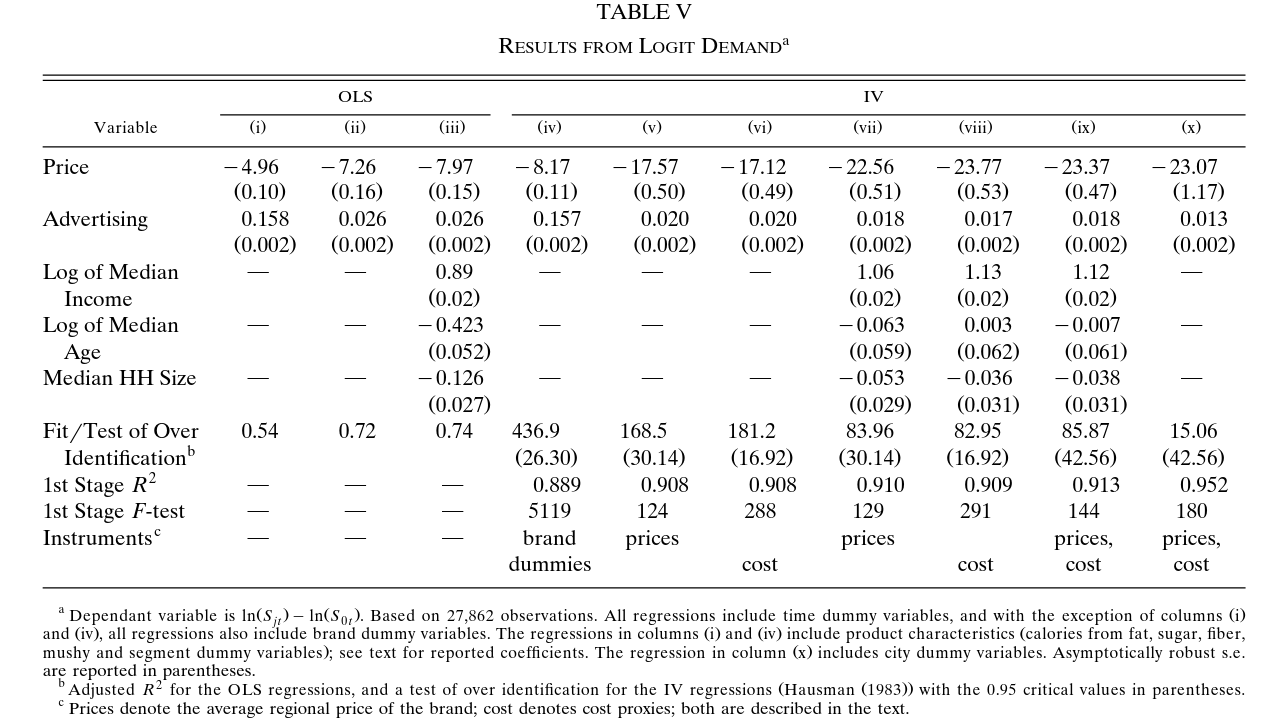
\includegraphics[width=\textwidth, keepaspectratio=true]{tab5.png}
   \end{frame}
   %
   \begin{frame}{Results---Full Model}
     \begin{center}
       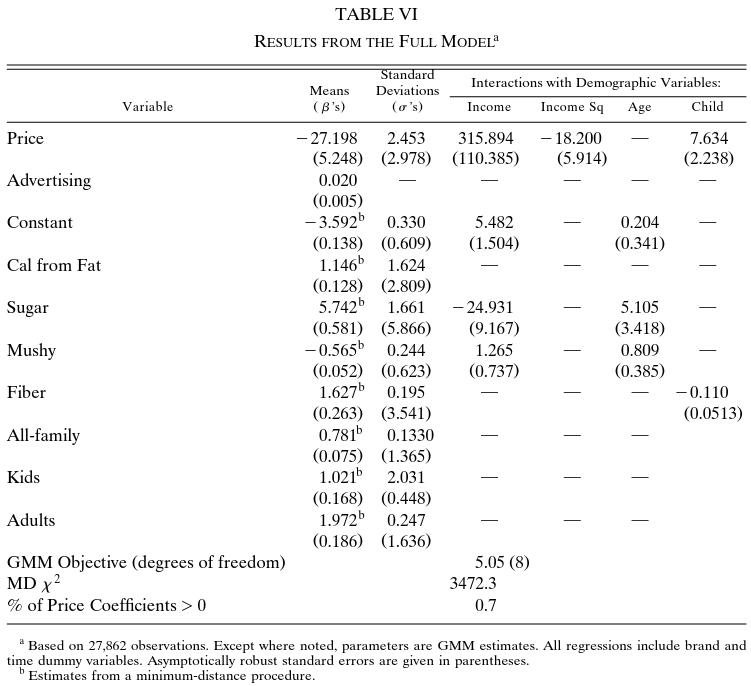
\includegraphics[height=0.9\textheight, keepaspectratio=true]{tab6.png}
     \end{center}
   \end{frame}
   %
   \begin{frame}{}
     \centering
     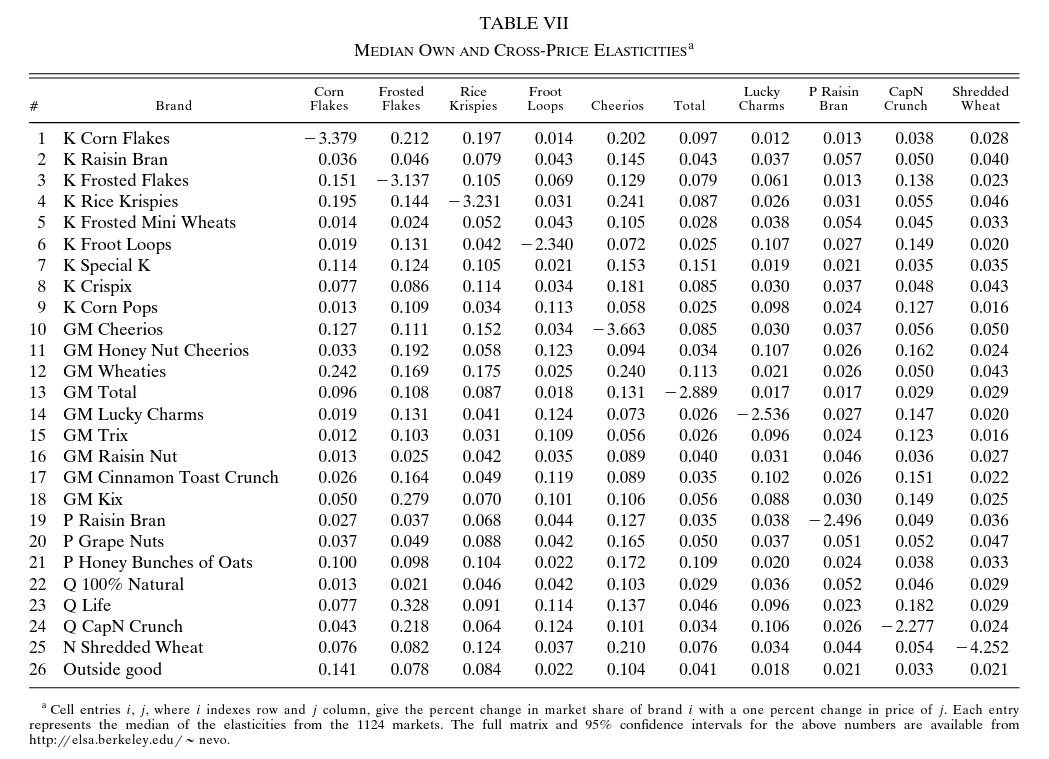
\includegraphics[width=\textwidth, keepaspectratio=true]{tab7.png}
   \end{frame}
   %
   \begin{frame}{Results: Firm Behavior---Nevo vs. Logit}
     \begin{center}
      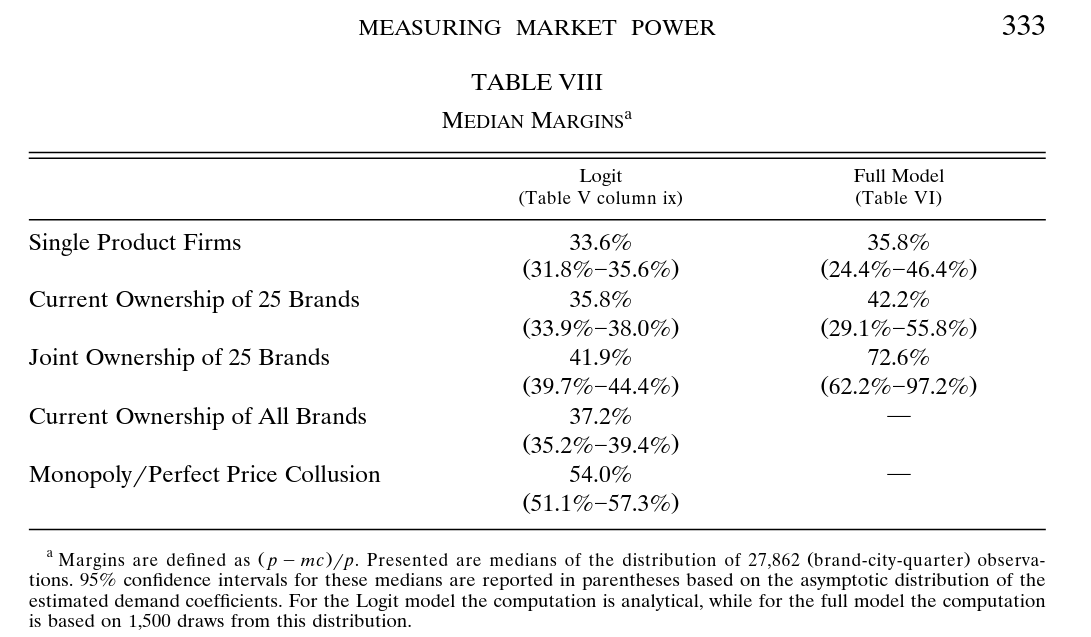
\includegraphics[width=\textwidth, keepaspectratio=true]{tab8.png} 
     \end{center}
   \end{frame}
   %
   \begin{frame}{Conclusions}
     \begin{quote}
       If we are willing to accept Nash-Bertrand as a benchmark of noncollusive pricing\ldots even with PCM greater than 45\%, prices in the industry are not a result of collusive behavior. The results rule out an extreme version of cooperative pricing\ldots the results in this paper do not rule out cooperate pricing between a subset of products \ldots
     \end{quote}
    \vfill 
     \begin{quote}
       As much as I would like to claim that this paper proves or disproves the FTC's case, I cannot\ldots the high observed PCM are primarily due to the firms' ability to maintain a portfolio of differentiated products\ldots
     \end{quote}
   \end{frame}
%
 \begin{frame}{Quick Aside---Transparency}
  \begin{quote} 
    A comment is in place about the realism of the assumption that consumers choose no more
than one brand. Many households buy more than one brand of cereal in each supermarket trip but
most people consume only one brand of cereal at a time, which is the relevant fact for this modeling
assumption. Nevertheless, if one is still unwilling to accept that this is a negligible phenomenon, then
this model can be viewed as an approximation to the true choice model. An alternative is to
explicitly model the choice of multiple products, or continuous quantities
(as in Dubin and McFadden (1984) or Hendel (1999)).
\end{quote}
\begin{quote}
  Treating the characteristics as predetermined, rather than reacting to demand
shocks, is as reasonable
(or unreasonable)
here as it was in previous work.
\end{quote}
 \end{frame}
 %
\end{document}
%%% Local Variables:
%%% mode: latex
%%% TeX-master: t
%%% End:
